\documentclass[tikz,border=3pt]{standalone}
\usepackage[utf8]{inputenc}
\usepackage[T1]{fontenc}
\usepackage{lmodern}
\renewcommand{\familydefault}{\sfdefault}
\usepackage{sansmath}\sansmath
\usepackage{chemfig}
\usepackage{pgfplots}\pgfplotsset{compat=1.18,/pgf/number format/use comma,/pgf/number format/1000 sep={.}}
\usetikzlibrary{arrows.meta,calc,positioning,decorations.pathmorphing,patterns}
% paleta del sitio
\definecolor{nar}{HTML}{E8680C}\definecolor{narc}{HTML}{FFB35C}\definecolor{hielo}{HTML}{FFF3E8}
\definecolor{tinta}{HTML}{1D1D1F}\definecolor{gris}{HTML}{6E6E73}\definecolor{lila}{HTML}{7C5CF0}
\definecolor{azul}{HTML}{2F6FD6}\definecolor{menta}{HTML}{17A673}\definecolor{coral}{HTML}{E8342A}
\begin{document}
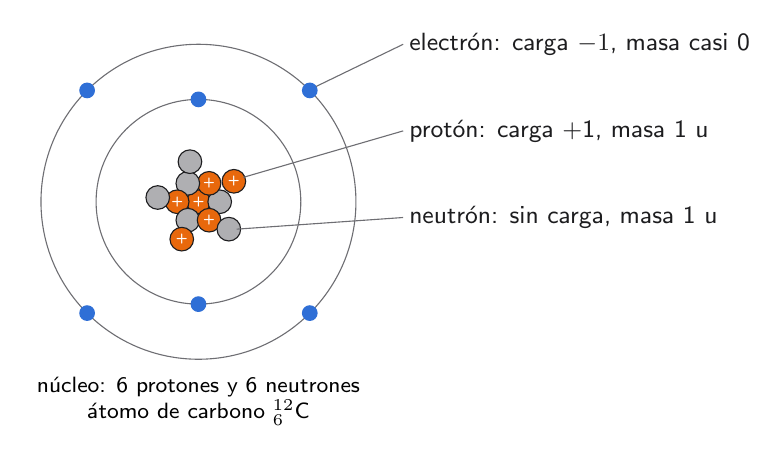
\begin{tikzpicture}[font=\small]
\draw[gris] (0,0) circle (1.3);
\draw[gris] (0,0) circle (2.0);
\fill[nar,draw=tinta,line width=0.4pt] (0,0) circle (0.15);
\node[text=white,font=\tiny\bfseries] at (0,0) {+};
\fill[gris!55,draw=tinta,line width=0.4pt] (0.27,0) circle (0.15);
\fill[nar,draw=tinta,line width=0.4pt] (0.135,0.234) circle (0.15);
\node[text=white,font=\tiny\bfseries] at (0.135,0.234) {+};
\fill[gris!55,draw=tinta,line width=0.4pt] (-0.135,0.234) circle (0.15);
\fill[nar,draw=tinta,line width=0.4pt] (-0.27,0) circle (0.15);
\node[text=white,font=\tiny\bfseries] at (-0.27,0) {+};
\fill[gris!55,draw=tinta,line width=0.4pt] (-0.135,-0.234) circle (0.15);
\fill[nar,draw=tinta,line width=0.4pt] (0.135,-0.234) circle (0.15);
\node[text=white,font=\tiny\bfseries] at (0.135,-0.234) {+};
\fill[nar,draw=tinta,line width=0.4pt] (0.45,0.26) circle (0.15);
\node[text=white,font=\tiny\bfseries] at (0.45,0.26) {+};
\fill[gris!55,draw=tinta,line width=0.4pt] (-0.108,0.509) circle (0.15);
\fill[gris!55,draw=tinta,line width=0.4pt] (-0.517,0.054) circle (0.15);
\fill[nar,draw=tinta,line width=0.4pt] (-0.212,-0.475) circle (0.15);
\node[text=white,font=\tiny\bfseries] at (-0.212,-0.475) {+};
\fill[gris!55,draw=tinta,line width=0.4pt] (0.386,-0.348) circle (0.15);
\fill[azul] (0,1.3) circle (0.1);
\fill[azul] (-0,-1.3) circle (0.1);
\fill[azul] (1.414,1.414) circle (0.1);
\fill[azul] (-1.414,1.414) circle (0.1);
\fill[azul] (-1.414,-1.414) circle (0.1);
\fill[azul] (1.414,-1.414) circle (0.1);
\draw[gris] (0.57,0.31) -- (2.6,0.9) node[anchor=west,text=tinta,align=left,inner sep=2pt] {protón: carga +1, masa 1 u};
\draw[gris] (0.486,-0.348) -- (2.6,-0.2) node[anchor=west,text=tinta,align=left,inner sep=2pt] {neutrón: sin carga, masa 1 u};
\draw[gris] (1.494,1.464) -- (2.6,2) node[anchor=west,text=tinta,align=left,inner sep=2pt] {electrón: carga $-1$, masa casi 0};
\node[anchor=north,align=center,font=\footnotesize] at (0,-2.1) {núcleo: 6 protones y 6 neutrones\\átomo de carbono ${}^{12}_{6}$C};

\end{tikzpicture}
\end{document}
